
\question{Replicate some of the results in ``The Colonial Origins of Comparative Development: An Empirical Investigation'' by Acemoglu, Johnson, and Robinson (AJR, 2001).}

%% ---- Part (i) ----
\textbf{(i)} I replicate columns (3), (5), and (6) of Table 2 in AJR (2001) by running OLS regressions of \texttt{loggdp} on \texttt{risk} with progressively more controls. The results are reported in Table~\ref{tab:ols}.

\begin{table}[H]
\centering
\caption{OLS Regressions -- Replication of AJR (2001) Table 2}
\label{tab:ols}

\begingroup
\centering
\begin{tabular}{lccc}
   \tabularnewline \midrule \midrule
   Dependent Variable: & \multicolumn{3}{c}{loggdp}\\
                & Column 2       & Column 5       & Column 6 \\   
   Model:       & (1)            & (2)            & (3)\\  
   \midrule
   \emph{Variables}\\
   risk         & 0.5162$^{***}$ & 0.4574$^{***}$ & 0.3956$^{***}$\\   
                & (0.0511)       & (0.0652)       & (0.0656)\\   
   latitude     &                & 1.710$^{**}$   & 0.9781\\   
                &                & (0.6836)       & (0.6364)\\   
   asia         &                &                & -0.6513$^{**}$\\   
                &                &                & (0.3117)\\   
   africa       &                &                & -0.8787$^{***}$\\   
                &                &                & (0.1550)\\   
   other        &                &                & 0.1027\\   
                &                &                & (0.2220)\\   
   \midrule
   \emph{Fit statistics}\\
   Observations & 64             & 64             & 64\\  
   R$^2$        & 0.52370        & 0.56378        & 0.70503\\  
   F-test       & 68.170         & 39.420         & 27.726\\  
   \midrule \midrule
   \multicolumn{4}{l}{\emph{Heteroskedasticity-robust standard-errors in parentheses}}\\
   \multicolumn{4}{l}{\emph{Signif. Codes: ***: 0.01, **: 0.05, *: 0.1}}\\
\end{tabular}
\par\endgroup



\end{table}

The coefficient on \texttt{risk} is positive and highly significant across all three specifications, declining from 0.52 to 0.40 as I add controls. This is consistent with the original paper: better institutions (higher protection against expropriation risk) are associated with higher GDP per capita.\\

%% ---- Part (ii) ----
\textbf{(ii)} I now run 2SLS regressions using \texttt{logmort0} (log settler mortality) as an instrument for \texttt{risk}. The second-stage results are reported in Table~\ref{tab:iv_second} and the first-stage results in Table~\ref{tab:iv_first}.

\begin{table}[H]
\centering
\caption{IV Regressions -- Second Stage}
\label{tab:iv_second}

\begingroup
\centering
\begin{tabular}{lccc}
   \tabularnewline \midrule \midrule
   Dependent Variable: & \multicolumn{3}{c}{loggdp}\\
                          & Column 2       & Column 5       & Column 6 \\   
   Model:                 & (1)            & (2)            & (3)\\  
   \midrule
   \emph{Variables}\\
   risk                   & 0.9295$^{***}$ & 0.9620$^{***}$ & 1.074$^{**}$\\   
                          & (0.1728)       & (0.2321)       & (0.5080)\\   
   latitude               &                & -0.4169        & -0.9940\\   
                          &                & (1.222)        & (1.814)\\   
   asia                   &                &                & -1.103$^{**}$\\   
                          &                &                & (0.5393)\\   
   africa                 &                &                & -0.4513\\   
                          &                &                & (0.3930)\\   
   other                  &                &                & -0.9532\\   
                          &                &                & (1.074)\\   
   \midrule
   \emph{Fit statistics}\\
   Observations           & 64             & 64             & 64\\  
   R$^2$                  & 0.46443        & 0.49370        & 0.58314\\  
   F-test                 & 53.766         & 29.740         & 16.227\\  
   Wald (1st stage), risk & 16.326         & 9.6982         & 3.1732\\  
   \midrule \midrule
   \multicolumn{4}{l}{\emph{Heteroskedasticity-robust standard-errors in parentheses}}\\
   \multicolumn{4}{l}{\emph{Signif. Codes: ***: 0.01, **: 0.05, *: 0.1}}\\
\end{tabular}
\par\endgroup



\end{table}

\begin{table}[H]
\centering
\caption{IV Regressions -- First Stage}
\label{tab:iv_first}

\begingroup
\centering
\begin{tabular}{lccc}
   \tabularnewline \midrule \midrule
   Dependent Variable: & \multicolumn{3}{c}{risk}\\
                & Column 2        & Column 5        & Column 6 \\   
   Model:       & (1)             & (2)             & (3)\\  
   \midrule
   \emph{Variables}\\
   logmort0     & -0.6133$^{***}$ & -0.5172$^{***}$ & -0.3499$^{*}$\\   
                & (0.1518)        & (0.1661)        & (0.1964)\\   
   latitude     &                 & 2.007           & 2.001\\   
                &                 & (1.356)         & (1.480)\\   
   asia         &                 &                 & 0.4674\\   
                &                 &                 & (0.5222)\\   
   africa       &                 &                 & -0.2567\\   
                &                 &                 & (0.3398)\\   
   other        &                 &                 & 1.046\\   
                &                 &                 & (0.7742)\\   
   \midrule
   \emph{Fit statistics}\\
   Observations & 64              & 64              & 64\\  
   R$^2$        & 0.27351         & 0.29967         & 0.33092\\  
   F-test       & 23.341          & 13.051          & 5.7373\\  
   \midrule \midrule
   \multicolumn{4}{l}{\emph{Heteroskedasticity-robust standard-errors in parentheses}}\\
   \multicolumn{4}{l}{\emph{Signif. Codes: ***: 0.01, **: 0.05, *: 0.1}}\\
\end{tabular}
\par\endgroup



\end{table}

The IV estimates of the coefficient on \texttt{risk} are substantially larger than the OLS estimates (0.93--1.07 vs.\ 0.40--0.52), suggesting that OLS is biased downward, possibly due to measurement error in institutional quality. The IV coefficient remains significant in all specifications.\\

%% ---- Part (iii) ----
\textbf{(iii)} The first-stage F-statistics (from Table~\ref{tab:iv_first}) are:
\begin{itemize}
    \item Column (3): $F = 23.34$
    \item Column (5): $F = 13.05$
    \item Column (6): $F = 5.74$
\end{itemize}

In the baseline specification without additional controls, the instrument is strong ($F \gg 10$). As I add controls (latitude, continent dummies), the first-stage F-statistic declines. In the full specification (Column 6), $F = 5.74 < 10$, falling below the rule-of-thumb threshold. This suggests that \texttt{logmort0} may be a weak instrument once I condition on the full set of controls, raising concerns about the reliability of the 2SLS estimates in that specification.\\

%% ---- Part (iv) ----
\textbf{(iv)} I implement the Anderson--Rubin (AR) test. For a given $\beta_0$, I construct:
\[
    y_i - x_i \beta_0 = z_i \delta + w_i' \alpha + u_i,
\]
where $z_i = \texttt{logmort0}$, $x_i = \texttt{risk}$, and $w_i$ includes latitude, asia, africa, and other (the controls from Column 6). Under the null $H_0: \beta = \beta_0$ and the exclusion restriction, $\delta = 0$. The AR statistic is the squared $t$-statistic for $\hat{\delta}$ (using heteroskedasticity-robust standard errors), which is asymptotically $\chi^2(1)$ under the null. The 5\% critical value is $\chi^2_{1,0.95} = 3.84$.

Figure~\ref{fig:ar_plot} plots the AR statistic as a function of $\beta_0$ over $[-10, 10]$ with a grid spacing of 0.01.

\begin{figure}[H]
    \centering
    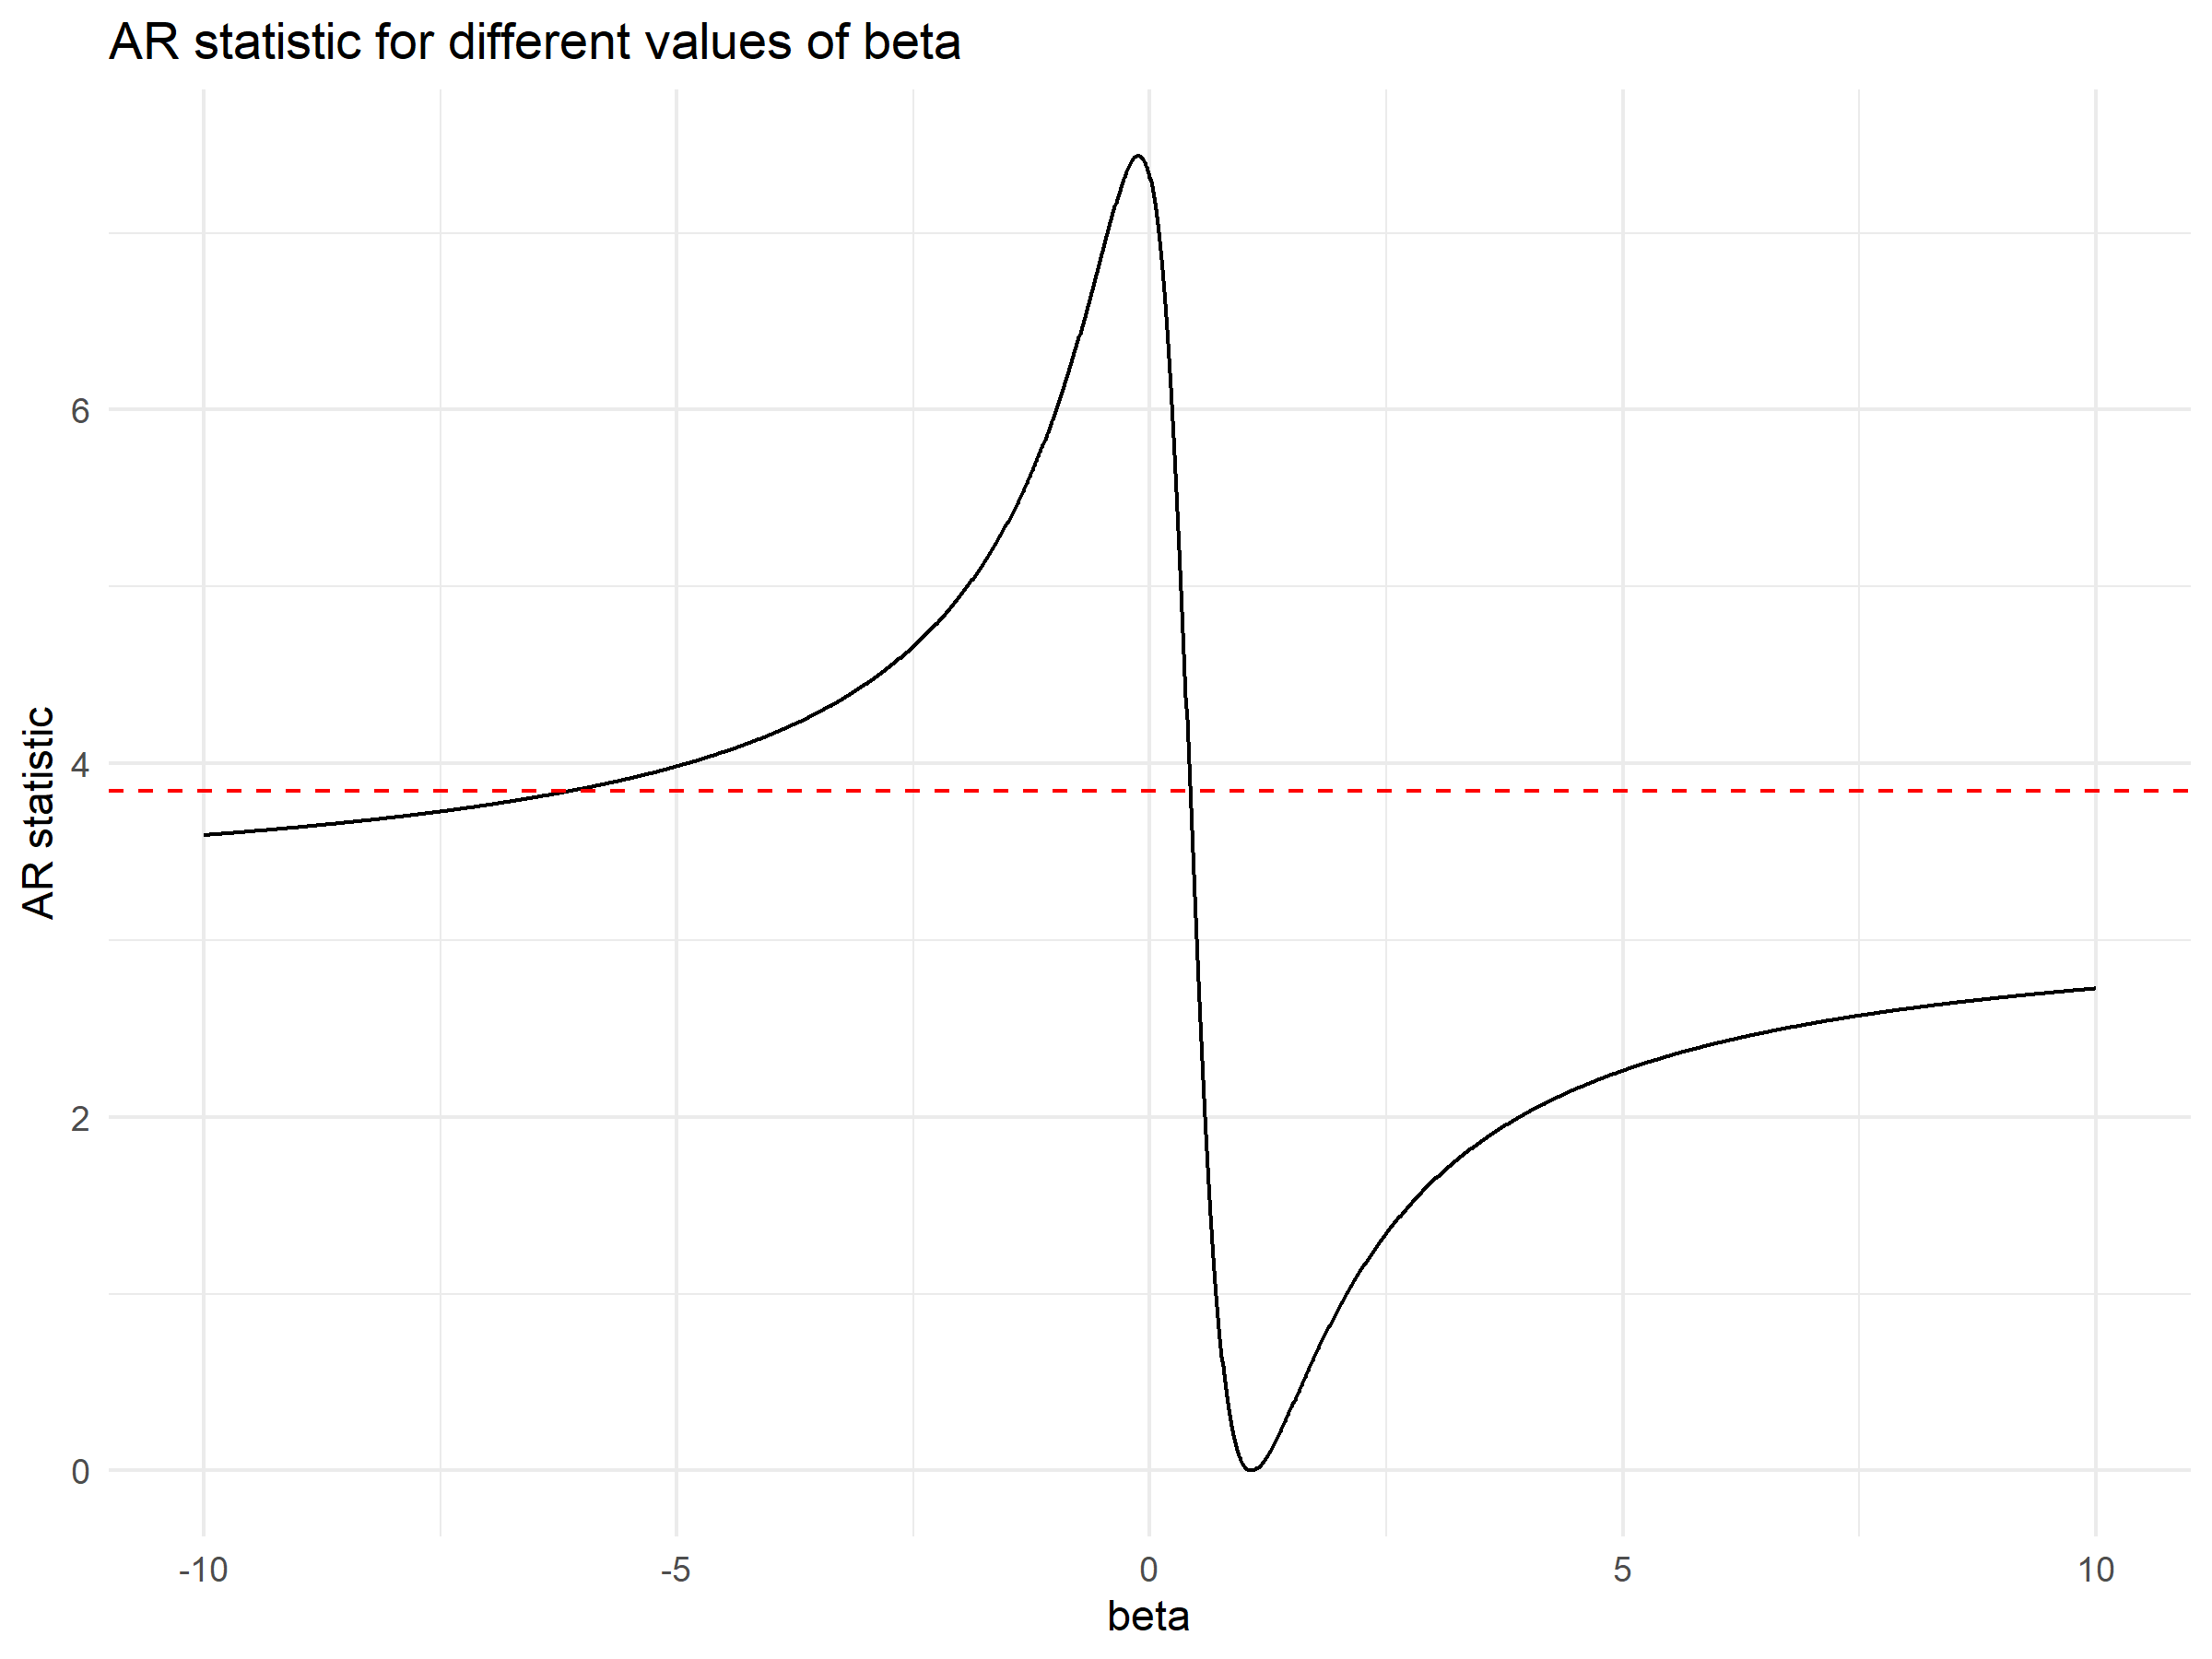
\includegraphics[width=0.85\textwidth]{Figures/AR_statistic_plot.png}
    \caption{Anderson--Rubin statistic as a function of $\beta$. The dashed red line marks the $\chi^2(1)$ critical value at the 5\% level (3.84).}
    \label{fig:ar_plot}
\end{figure}

The 95\% AR confidence set for $\beta$ consists of all values where the AR statistic falls below 3.84. From the plot and grid search, this set is:
\[
    \text{CS}_{95\%} = [-10, -6.16] \cup [0.43, 10].
\]

The IV estimates from \ref{tab:iv_second} lie in the confidence interval.\\

This is a \emph{disconnected} confidence set, which is caused by weak instruments. The AR test is robust to weak instruments (unlike standard Wald-based inference), and the wide, disconnected confidence set reflects the substantial uncertainty about $\beta$ when the instrument is weak in the full specification. Notably, the set includes both large negative and large positive values of $\beta$, indicating that I cannot precisely pin down the effect of institutions on GDP when using the full set of controls. The 2SLS point estimate of $\hat{\beta} = 1.074$ falls within the confidence set, but so do many other values, including negative ones. This underscores the importance of instrument strength for reliable inference.